\documentclass{beamer}

\usepackage[italian]{babel}
\usepackage{graphicx}
\usepackage{url}
\usepackage{hyperref}
\usepackage{soul}
\usepackage{tikz}
\usepackage{listings}
\usepackage{xcolor}
\usepackage{algorithm}
\usepackage{multicol}
\usepackage{textcomp}
\usepackage[noend]{algpseudocode}

\newcommand{\code}[1]{{\fontfamily{lmtt}\selectfont#1}}

\setbeamertemplate{navigation symbols}{}
\usetheme{default}
\usecolortheme{Nord}

\title{CoderFarm - Corso avanzato}
\subtitle{Lezione 2}
\author{Lorenzo Ferrari, Davide Bartoli}
\date{\today}

\begin{document}

\begin{frame}
    \titlepage
\end{frame}

\section{Problemi}

\begin{frame}{Lotteria}{}
    \begin{exampleblock}{Edoardo e la lotteria}
        Nel lotto da Cesena bisogna scegliere $n \leq 20$ numeri da $1$ a $m \leq 200 \ 000$. Una lista \`e fortunata se e solo se ogni numero \`e almeno il doppo del precedente. Contare quante liste fortunate esistono e stampare la risposta modulo $10^9 + 7$.
    \end{exampleblock}
    \small{ \underline{\url{https://training.olinfo.it/\#/task/lotteria/statement}}}
    \pause
    \begin{itemize}
        \item idee?
        \pause
        \item \st{se lo vediamo in questa lezione evidentemente \`e una \texttt{dp}}
        \pause
        \item sia $dp[i][j]$ il numero di liste di $i$ elementi il cui ultimo elemento \`e $j$
        \pause
        \item ovviamente $dp[1][j] = 1 \ \forall j $
        \item la risposta \`e $dp[n][m] + dp[n][m-1] + \dots + dp[n][1]$
    \end{itemize}
\end{frame}

\begin{frame}{Lotteria}{}
    \begin{itemize}
        \item supponiamo di avere calcolato $dp[i'][j']$ per ogni $i' < i$ e $j' < j$
        \pause
        \item se l'$i$-esimo elemento \`e $j$ e l'$(i-1)$-esimo elemento \`e $j'$, deve valere $j \geq 2 j'$, quindi $j' \leq \lfloor j / 2 \rfloor$
    \end{itemize}
    \pause
    \vfill
    \[
        dp[i][j] = dp[i-1][1] + dp[i-1][2] + \dots + dp[i-1][j/2]
    \]
    \pause
    \vfill
    \begin{itemize}
        \item implementiamo questa soluzione
    \end{itemize}
\end{frame}

\begin{frame}
    \makebox[\textwidth]{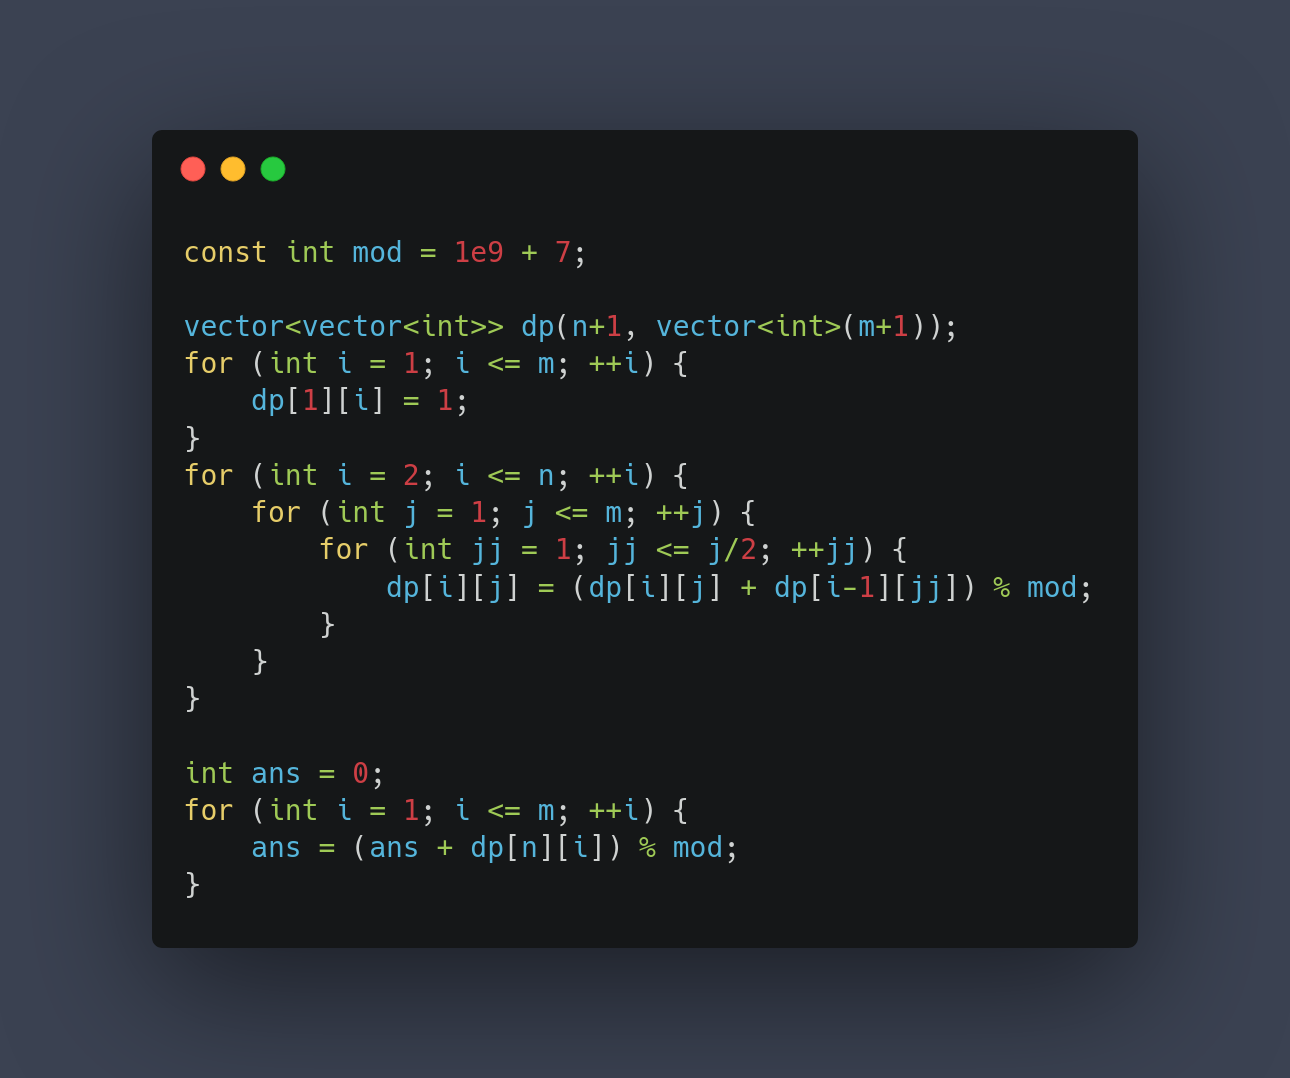
\includegraphics[scale=.25]{./img/lotteria_70.png}}
\end{frame}

\begin{frame}{Lotteria}{Complessit\`a}
    \begin{itemize}
        \item $O(n m)$ stati
        \item $O(m)$ per transizione
        \pause
        \item $O(n m^2)$ complessit\`a totale
    \end{itemize}
    \pause
    La soluzione attuale prende $70/100$ punti.
\end{frame}

\begin{frame}{Lottera}{Ottimizzazione}
    Come ottimizzare?
    \pause
    \begin{itemize}
        \item per calcolare $dp[i][j]$ e $dp[i][j+1]$ la maggior parte dei valori che sommiamo sono uguali
        \pause
        \item in particolare, $dp[i][j+1]$ differisce da $dp[i][j]$ solo per i valori $dp[i-1][x]$ con $j/2 < x \leq (j+1)/2$ (al massimo un valore)
        \pause
        \item possiamo ridurre il costo della transizione a $O(1)$!
    \end{itemize}
\end{frame}

\begin{frame}
    \makebox[\textwidth]{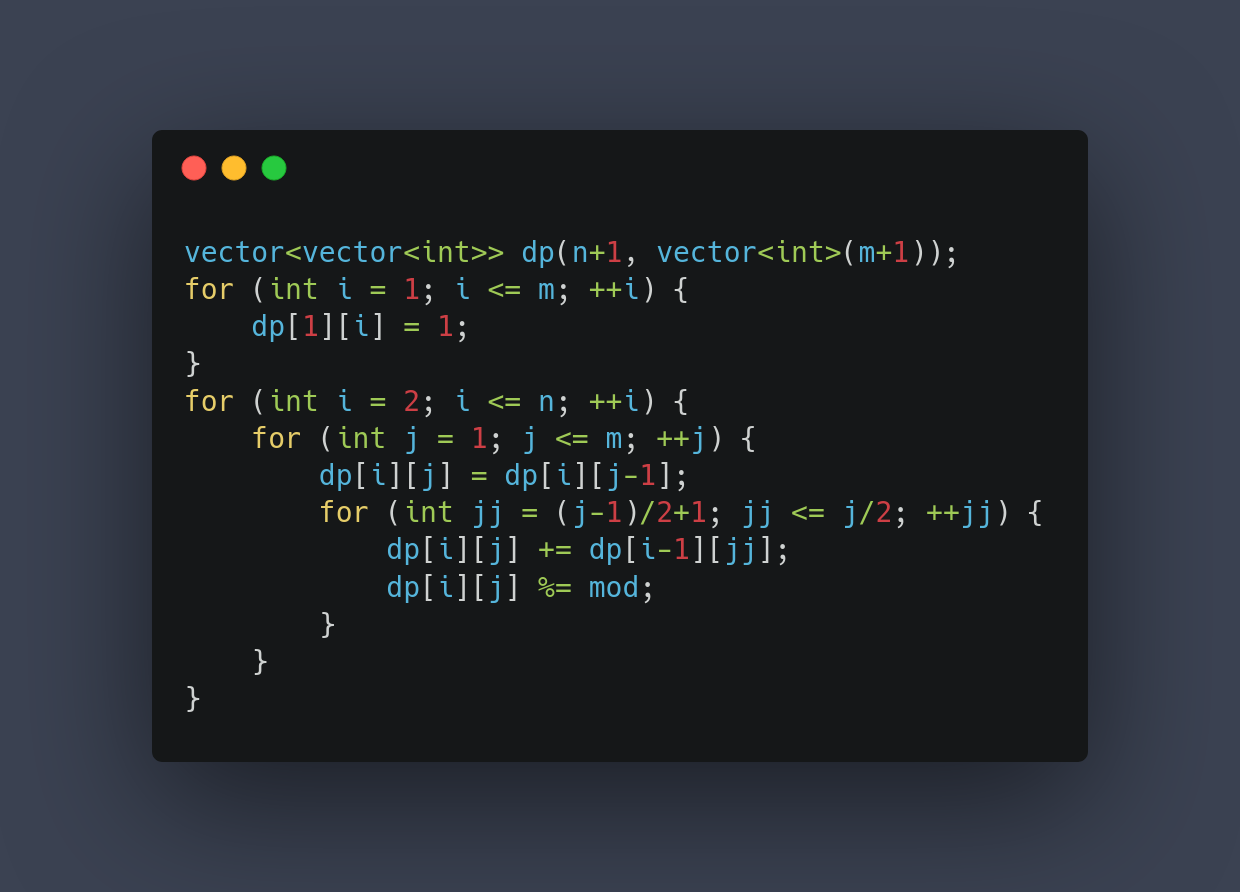
\includegraphics[scale=.30]{./img/lotteria_100_senza_prefix.png}}
\end{frame}

\begin{frame}[fragile]{Lotteria}{Somme prefisse}
    Un'alternativa \`e salvarsi le \textbf{somme prefisse}
    \pause
    \begin{block}{}
        \begin{itemize}
            \item dato un array $a[0], a[1], \dots, a[n-1]$, l'array delle somme prefisse di $a$ \`e un array $prf$ tale che $prf[i] = a[0] + a[1] + \dots + a[i]$
            \pause
        \item $prf[0] = a[0]$
        \item $prf[i] = prf[i-1] + a[i] \ \forall i > 0$
        \end{itemize}
    \end{block}
    \pause
    Se $a$ non cambia mai, possiamo trovare la somma degli $a[i]$ con $l \leq i \leq r$ in $O(1)$ come $sum(l, r) = prf[r] - prf[l-1]$
    \vfill
    Nel nostro caso $l = 0, r = \lfloor j/2 \rfloor$
\end{frame}

\begin{frame}
    \makebox[\textwidth]{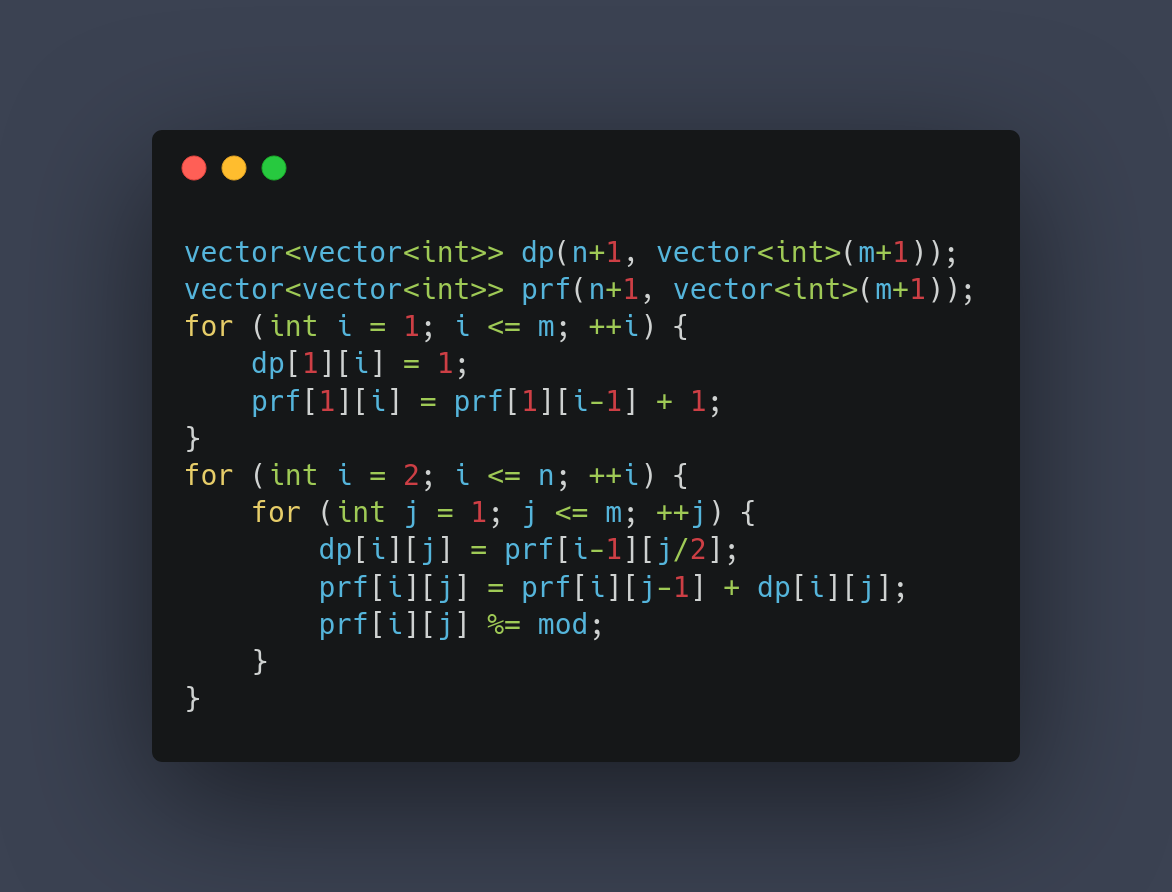
\includegraphics[scale=.30]{./img/lotteria_prefix_sums.png}}
\end{frame}

% momento domande? se capiscono tutto è stonks, ma non è scontato

\begin{frame}{Bitmask dp}{Matching}
    \begin{exampleblock}{Matching}
        Ci sono $N$ uomini e $N$ donne ($N \leq 20$), entrambi numerati $\, 2, \dots, N$. Data una matrice $a$, l'uomo $i$ e la donna $j$ sono compatibili sse $a_{i,j} = 1$.
        Vuoi fare $N$ coppie, ognuna costituita da un uomo e una donna compatibili e inoltre ognuno deve appartenere a esattamente una coppia. \\
        Trova in quando modi puoi formare le $N$ coppie modulo $10^9 + 7$.
    \end{exampleblock}
    \small{\underline{\url{https://atcoder.jp/contests/dp/tasks/dp_o}}}
    \pause
    \begin{itemize}
        \item quali potrebbero essere gli stati della nostra dp?
        \pause
        \item un set $S$ di uomini ``assegnati'' alle prime $j$ donne
        \item $dp[S][j]$: numero di modi per farlo
        \pause
        \item per le transizioni possiamo pensare a chi va in coppia con la donna $j$, l'ultima del prefisso
    \end{itemize}
\end{frame}

\begin{frame}{Bitmask dp}{Matching}
    In particolare
    \[
        dp[S][j] = \sum_{i=1}^{N}{ \left( dp[S \backslash \{i\}][j-1] \text{ se } a_{i,j} = 1 \right) }
    \]
    \pause
    Stiamo contando tutti gli assegnamenti esattamente una volta: se assegnamo la donna $j$ a diversi $i$ non abbiamo sovrapposizioni
    \pause
    \bigbreak

    La risposta \`e $dp[\{1, 2, \dots, N\}][N]$
\end{frame}

\begin{frame}{Bitmask dp}{Matching}
    \begin{itemize}
        \item come si implementa?
        \pause
        \item ci serve un modo per rappresentare un set $S$ con un intero
        \pause
    \item possiamo rappresentare $S$ come un intero $mask$ a $N$ bit dove il bit $i$-esimo \`e $1$ se e solo se $i \in S$
        \pause
        \item le operazioni bitwise ci consentono di effettuare efficientemente operazioni come inserire/rimuovere un elemento e controllare se un elemento \`e presente
    \end{itemize}
\end{frame}

\begin{frame}[fragile]{Bitmask dp}{Matching}
    \begin{itemize}
        \item l'elemento $i$-esimo \`e rappresentato dalla potenza $2^i$ con $0 \leq i \leq N-1$
        \pause
    \item \verb|if (mask & (1 << i))| controlla se $i$ \`e presente in $mask$
    \item \texttt{mask |= (1 << i)} inseriesce $i$ in $mask$
    \item \verb|mask &= ~(1 << i)| rimuove $i$ da $mask$
    \item \verb|mask ^= (1 << i)| cambia lo stato di $i$ in $mask$: se $i$ \`e presente lo rimuove, altrimenti lo inserisce
    \end{itemize}
\end{frame}

\begin{frame}
    \makebox[\textwidth]{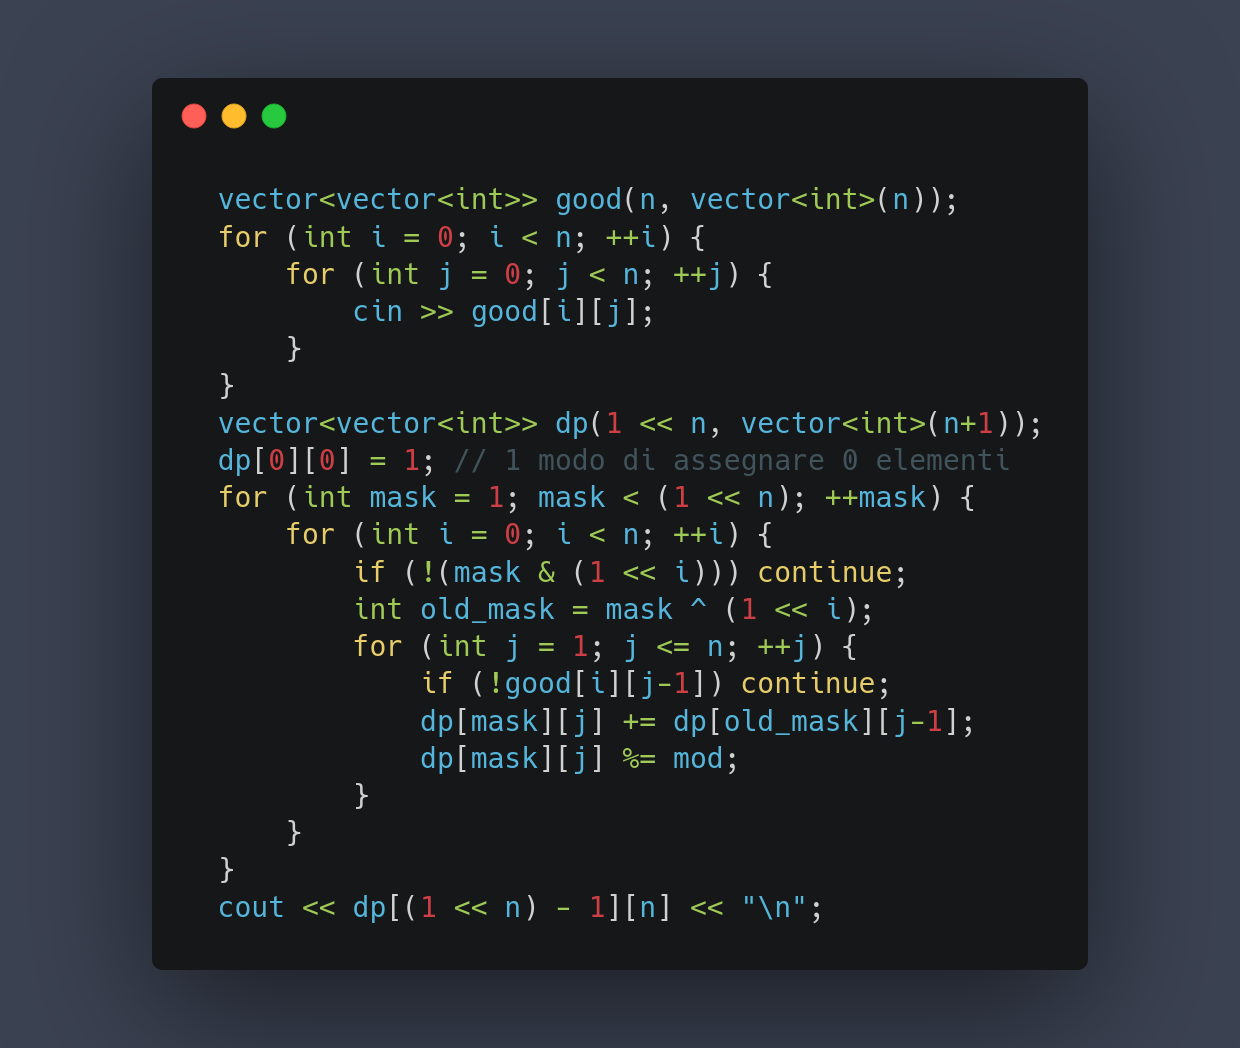
\includegraphics[scale=.25]{./img/matching.png}}
\end{frame}

\begingroup
\setbeamertemplate{navigation symbols}{}
\begin{frame}[plain, fragile]{Matching}{Complessit\`a}
    Un problema (praticamente) identico \`e \href{https://training.olinfo.it/\#/task/ois_dristor2/statement}{\underline{ois\_dristor2}}\footnote{che nessuna squadra ha risolto in gara (no neanch'io che sto scrivendo) :P}
    \pause
    \begin{exampleblock}{Lost in Dristor 2}
        Dati $N \leq 14$, $M \leq 100$ e una matrice $N \times M$ che indica se elementi del primo insieme sono a coppie compatibili con elementi del secondo insieme, conta quanti max matching (matching con il massimo numero di coppie) esistono.
    \end{exampleblock}
    \pause
    \begin{itemize}
        \item in questo caso dobbiamo anche contare il numero di elementi in $mask$
        \pause
        \item si pu\`o fare in $O(1)$ con \verb|__builtin_popcount(mask)|, che restituisce il numero di bit $1$ nella rappresentazione binaria di $mask$
        \pause
    \item divertitevi a implementarlo (\`e molto pulito)
    \end{itemize}
\end{frame}
\endgroup

\begin{frame}{Problemi addizionali}{Implementateli che vi fa bene}
    \underline{\url{https://training.olinfo.it/\#/task/ois_dristor2/statement}}
    \underline{\url{https://training.olinfo.it/\#/task/ois_police4/statement}}
    \underline{\url{https://atcoder.jp/contests/dp/tasks}}
    \underline{\url{https://cses.fi/problemset/}}
\end{frame}

\end{document}
